\chapter{Double Integrals in Other Coordinate Systems}

\section{Double Integrals in Other Coordinate Systems}
% \index{double integral! polar coordinates}
\index{polar double integrals}
Consider a region composed of a semi-circular ring (see figure \ref{
fig:semicircle}). Describing the region in Cartesian coordinates is 
complicated; you would have to split it into three regions. However, in polar coordinates, we can describe the whole region in one statement:
$$\textit{D} = \{(r, \theta)\text{ }|\text{ }1 \leq r \leq 4,\text{ }0 \leq 
\theta \leq \pi\}$$

\begin{figure}[H]
    \centering
    \begin{tikzpicture}
    \begin{axis}[xlabel = $x$, ylabel = $y$, xmin = -5, xmax = 5, ymin = -1, 
    ymax = 5, axis lines = center, unit vector ratio*=1 1 1]
        \addplot[name path = A, domain = -4:4, blue, thick, samples = 100] {
        sqrt(16 - x^2)};
        \addplot[name path = B, domain = -1:1, blue, thick, samples = 100] {
        sqrt(1-x^2)};
        \addplot[blue, thick, domain = -4:-1]{0};
        \addplot[blue, thick, domain = 1:4]{0};
        \addplot[blue!30, opacity = 0.4] fill between[of = A and B];
    \end{axis}
\end{tikzpicture}
    \caption{A semi-circular ring}
    \label{fig:semicircle}
\end{figure}

There are many instances where a region is simpler to describe in polar 
coordinates, so how do we take double integrals in polar coordinates? Suppose 
we want to integrate some function, $f(x,y)$, over a \index{polar rectangle}polar rectangle described 
by $\textit{D} = \{(r, \theta)\text{ }|\text{ }a \leq r \leq b,\text{ }\alpha 
\leq \theta \leq \beta \}$ (see figure \ref{fig:polar_rect}). Similar to 
Cartesian coordinates, we can divide this region into many smaller polar 
rectangles, with each subrectangle defined by $\textit{D}_{ij} = \{(r, \theta)
\text{ }|\text{ }r_{i-1} \leq r \leq r_i,\text{ }\theta_{i - 1} \leq \theta 
\leq \theta_i\}$. The center of each subrectangle has polar coordinates $(
r_i^*, \theta_j^*)$, where:
$$r_i^* = \frac{1}{2} \left( r_{i - 1} + r_i \right)$$
$$\theta_j^* = \frac{1}{2} \left( \theta_{j - 1} + \theta_j \right)$$ 

\begin{figure}[H]
    \centering
    \begin{tikzpicture}
    \begin{axis}[xlabel = $x$, ylabel = $y$, xmin = -0.5, xmax = 4, 
    ymin = -0.5, ymax = 4, axis lines = center, unit vector ratio*=1 1 1]
        \addplot[name path = A, domain = 2:3.464, blue, thick, samples = 100] {
        sqrt(16 - x^2)};
        \addplot[name path = B, domain = 0.5:0.866, blue, thick, samples = 100]
         {sqrt(1-x^2)};
        \draw[blue, thick] (2, 3.464) -- (0.5, 0.866);
        \draw[blue, thick] (3.464, 2) -- (0.866, 0.5);
        \addplot[blue!30, opacity = 0.4] fill between[of = A and B];
        \draw[dashed] (0,0) -- (2, 3.464) node[left, font = \scriptsize, 
        yshift = -1cm, xshift = -0.5cm] {$\theta = \beta$};
        \draw[dashed] (0,0) -- (3.464, 2) node[right, font = \scriptsize, 
        yshift = -1cm, xshift = -1.5cm] {$\theta = \alpha$};
        \draw[-latex] (0.8, 0) arc [start angle = 0, end angle = 30, 
        x radius = 0.8cm, y radius = 0.8cm] node[right, font = \scriptsize, 
        yshift = -0.1cm, xshift = 0.05cm] {$\alpha$};
        \draw[-latex] (0.4, 0) arc [start angle = 0, end angle = 60, 
        x radius = 0.4cm, y radius = 0.4cm] node[right, font = \scriptsize, 
        xshift = 0.03cm, yshift = 0.1cm] {$\beta$};
        \node[font = \scriptsize] at (1., 0.9) {$r = a$};
        \node[font = \scriptsize] at (3.1, 3.1) {$r = b$};
    \end{axis}
\end{tikzpicture}
    \caption{A polar rectangle described by $\textit{D} = \{(r, \theta)\text{ }
    |\text{ }a \leq r \leq b,\text{ }\alpha \leq \theta \leq \beta \}$}
    \label{fig:polar_rect}
\end{figure}

Each subrectangle is a larger radius sector minus a smaller radius sector, each
with the same central angle, $\Delta \theta = \theta_{j} - \theta_{j - 1}$. 
The total area of each subrectangle is given by:
$$\Delta A_i = \frac{1}{2}\left(r_i \right)^2 \Delta \theta - \frac{1}{2} 
\left( r_{i - 1} \right)^2 \Delta \theta = \frac{1}{2} \left( r_i^2 - r_{i - 1}
^2 \right) \Delta \theta$$

Substituting $\left( r_i^2 - r_{i - 1}^2 \right) = \left( r_i + r_{i - 1} 
\right) \left( r_i - r_{i - 1} \right)$, we see that:
$$\Delta A_i = \frac{1}{2} \left( r_i + r_{i - 1} \right) \left( r_i - r_{i - 1
} \right) \Delta \theta$$

Recall that we have defined $r_i^* = \frac{1}{2} \left(r_{i - 1} + r_i 
\right)$. Additionally, $\Delta r = r_{i} - r_{i - 1}$. Substituting this, we 
find a simplified expression for the area of each subrectangle:
$$\Delta A_i = r_i^* \Delta r \Delta \theta$$

Therefore, the Riemann sum of $f(x,y)$ over the region is:
$$\sum_{i = 1}^n \sum_{j = 1}^n f(r_i^* \cos{\theta_j^*}, r_i^* \sin{\theta_j^*
}) \Delta A_i$$

(Recall that to convert from Cartesian to polar coordinates, we use $x = r\cos{
\theta}$ and $y = r\sin{\theta}$). Substituting for $\Delta A_i$:
$$= \sum_{i = 1}^n \sum_{j = 1}^n f(r_i^* \cos{\theta_j^*}, r_i^* \sin{\theta_j
^*}) r_i^* \Delta r \Delta \theta$$

Taking the limit as $n \to \infty$, the Riemann sum becomes the double integral:
$$\int_{\alpha}^{\beta} \int_a^b f(r\cos{\theta}, r\sin{\theta}) r\,dr\,d
\theta$$

Therefore, if $f$ is continuous on the polar rectangle $a \leq r \leq b$, 
$\alpha \leq \theta \leq \beta$, then:
$$\iint_{\textit{D}} f(x,y)\,dA = \int_{\alpha}^{\beta} \int_a^b f(r\cos{\theta
}, r\sin{\theta})r\,dr\,d\theta$$

\textbf{Example}: Evaluate $\iint_{\textit{D}} x^2y\,dA$, where \textit{D} is 
the semi-circle shown below. 

\begin{center}
\begin{tikzpicture}
    \begin{axis}[xlabel = $x$, ylabel = $y$, xmin = -5.5, xmax = 5.5, ymin = 
    -0.5, ymax = 5.5, axis lines = center, unit vector ratio*=1 1 1]
        \addplot[name path = A, blue, thick, domain = -5:5, samples = 100]{
        sqrt(25-x^2)}; 
        \addplot[name path = B, blue, thick, domain = -5:5, samples = 100]{0};
        \addplot[fill = blue!30, opacity = 0.4] fill between [of = A and B];
        \node[] at (2, 2) {$D$};
    \end{axis}
\end{tikzpicture}
\end{center}

\textbf{Solution}: Since the region is a semi-circle with radius 5, we can 
describe \textit{D} as $\textit{D} = \{(r, \theta)\text{ }|\text{ }0 \leq r 
\leq 5,\text{ }0 \leq \theta \leq \pi\}$. Therefore, 
$$\iint_{\textit{D}} x^2y\,dA = \int_0^{\pi} \int_0^5 \left(r\cos{\theta} 
\right)^2 \left(r \sin{\theta}\right) r\,d\theta\,dr$$
$$= \int_0^{\pi} \int_0^5 r^4 \cos^2{\theta} \sin{\theta}\,dr\,d\theta$$
$$= \int_0^{\pi} \cos^2{\theta} \sin{\theta} \left[ \frac{1}{5}r^5 \right]_{r 
= 0}^{r = 5}\,d\theta$$
$$=\int_0^{\pi} \cos^2{\theta} \sin{\theta} \frac{5^5}{5}\,d\theta = 625 \int_0
^{\pi} \cos^2{\theta}\sin{\theta}\,d\theta$$

Using $u$-substitution, let $u = \cos{\theta}$. Then $-du = \sin{\theta} d
\theta$, therefore:
$$625 \int_0^{\pi} \cos^2{\theta}\sin{\theta}\,d\theta = 625 \int_{\theta = 0}^
{\theta = \pi} -u^2\,du$$
$$= -625 \frac{1}{3}u^3|_{\theta = 0}^{\theta = \pi} = -625 \frac{1}{3} \left( 
\cos^3{\theta} \right)|_{\theta = 0}^{\theta = \pi}$$
$$= -\frac{625}{3} \left[ (-1)^3 - (1)^3 \right] = -\frac{625}{3} \left(-2 
\right) = \frac{1250}{3}$$

\begin{Exercise}[title = {Changing to Polar Coordinates}, label = polarmulti3]
Evaluate the following iterated integrals by converting to polar coordinates:
\begin{enumerate}
    \item $\int_0^2 \int_0^{\sqrt{4 - x^2}} e^{-x^2 - y^2}\,dy\,dx$
    \item $\int_0^{1/2} \int_{\sqrt{3}y}^{\sqrt{1 - y^2}} xy^2\,dx\,dy$
    \item $\int_0^2 \int_0^{\sqrt{2x - x^2}} \sqrt{x^2 + y^2}\,dy\,dx$
\end{enumerate}
\vspace{130mm}
\end{Exercise}

\begin{Answer}[ref = polarmulti3]
\begin{enumerate}
    \item Let us visualize the region in the $xy$-plane:
    
    \begin{tikzpicture}
        \begin{axis}[axis lines = center, xmin = -0.5, xmax = 2.5, ymin = -0.5,
        ymax = 2.5, xlabel = $x$, ylabel = $y$, xtick = {2}, ytick = {2}, 
        unit vector ratio = 1 1 1]
            \addplot[name path = A, blue, thick, domain = 0:2, samples = 100]{
            sqrt(4 - x^2)}; 
            \addplot[name path = B, blue, thick, domain = 0:2]{0};
            \draw[blue, thick] (0,0) -- (0,2);
            \addplot[fill=blue!30, opacity = 0.4] fill between [of = A and B];
        \end{axis}
    \end{tikzpicture}

    The region is a quarter-circle that can be described with $\textit{D} = \{(
    r, \theta)\text{ }|\text{ }0 \leq r \leq 2,\text{ }0 \leq \theta \leq \pi/2
    \}$. We can then rewrite the integral in polar coordinates:
    $$\int_0^2 \int_0^{\sqrt{4 - x^2}} e^{-x^2 - y^2}\,dy\,dx = \int_0^{\pi/2} 
    \int_0^2 r e^{-r^2}\,dr\,d\theta$$
    $$= \int_0^{\pi/2} \left[ -\frac{1}{2}e^{-r^2}\right]_{r = 0}^{r = 2}\,d
    \theta = \int_0^{\pi/2} \left( -\frac{1}{2} \right) \left[ e^{-4} - 1 
    \right]\,d\theta$$
    $$= \frac{1}{2} \int_0^{\pi/2} 1 - e^{-4}\,d\theta = \frac{1}{2} \left(1 - 
    \frac{1}{e^4} \right) \int_0^{\pi/2} 1\,d\theta$$
    $$= \frac{1}{2} \left( 1 - \frac{1}{e^4} \right) \theta|_{\theta = 0}^{
    \theta = \pi/2} = \frac{\pi}{4} \left( 1 - \frac{1}{e^4} \right)$$

    \item The region is bounded by the $x$-axis, the line $y = x/\sqrt{3}$, and
    the circle $x^2 + y^2 = 1$:

    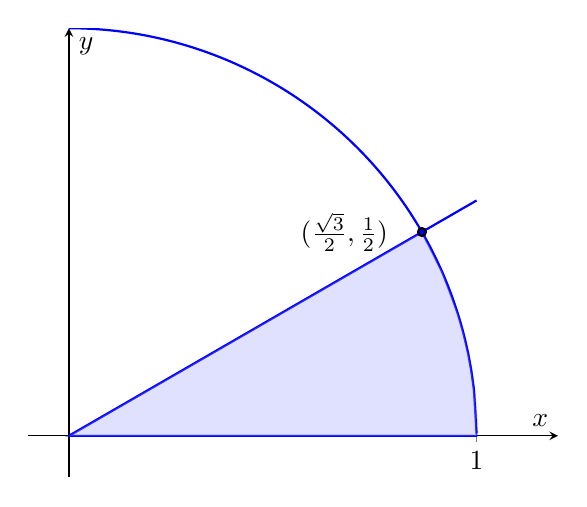
\begin{tikzpicture}
        \begin{axis}[axis lines = center, xtick = {1}, ytick = \empty, 
        ymin = -0.1, ymax = 1, xmin = -0.1, xmax = 1.2, xlabel = $x$, 
        ylabel = $y$, unit vector ratio = 1 1 1]
            \addplot[blue, thick, domain = 0:1, samples = 150]{sqrt(1-x^2)};
            \addplot[blue, thick, domain = 0:1]{x/sqrt(3)};
            \addplot[blue, thick, domain = 0:1]{0};
            \filldraw[blue, thick, fill = blue!30, opacity = 0.4] (0,0) -- 
            (1, 0) -- (0.99875, 0.05) -- (0.99499, 0.1) -- (0.98869, 0.15) -- 
            (0.9798, 0.2) -- (0.96825, 0.25) -- (0.95394, 0.3) -- 
            (0.91652, 0.4) -- (0.866, 0.5) -- cycle;
            \draw[black, thick, fill = blue] (0.866, 0.5) circle (0.05cm) node[
            black, left, xshift = -0.3cm] {$(\frac{\sqrt{3}}{2}, \frac{1}{2})$};
        \end{axis}
    \end{tikzpicture}

    We see that the region defined in polar coordinates is $\textit{D} = \{(r, 
    \theta)\text{ }|\text{ }0 \leq r \leq 1,\text{ }0 \leq \theta \leq \pi/6\}$
    . And therefore:
    $$\int_0^{1/2} \int_{\sqrt{3}y}^{\sqrt{1 - y^2}} xy^2\,dx\,dy = \int_0^{
    \pi/6} \int_0^1 r \left( r \cos{\theta} \right) \left(r \sin{\theta} 
    \right)^2\,dr\,d\theta$$
    $$= \int_0^{\pi/6} \left[ \cos{\theta} \sin^2{\theta} \right]\,d\theta 
    \cdot \int_0^1 r^4 \,dr$$
    $$= \left( \frac{1}{3}\sin^3{\theta}|_{\theta = 0}^{\theta = \pi/6} \right) 
    \cdot \left( \frac{1}{5} r^5 |_{r = 0}^{r = 1}\right)$$
    $$= \frac{1}{15} \cdot \left( \frac{1}{2} \right)^3 = \frac{1}{120}$$

    \item Visualizing the region:
    
    \begin{tikzpicture}
        \begin{axis}[axis lines = center, xtick = {1, 2}, ytick = {1}, 
        xmin = -0.2, xmax = 2.2, ymin = -0.2, ymax = 1.2, unit vector ratio = 
        1 1 1, xlabel = $x$, ylabel = $y$]
            \addplot[name path = A, blue, thick, domain = 0:2, samples = 150]{
            sqrt(2*x - x^2)};
            \addplot[name path = B, blue, thick, domain = 0:2]{0};
            \addplot[blue, fill = blue!30, opacity = 0.4] fill between [
            of = A and B];
        \end{axis}
    \end{tikzpicture}

    We see that the region is the top half of a circle of radius 1 centered at 
    (1, 0). In polar coordinates, this region is $\textit{D} = \{(r, \theta)
    \text{ }|\text{ }0 \leq r \leq 2\cos{\theta}, 0 \leq \theta \leq \pi/2\}$. 
    And therefore:
    $$\int_0^2 \int_0^{\sqrt{2x - x^2}} \sqrt{x^2 + y^2}\,dy\,dx = \int_0^{\pi/
    2} \int_0^{2\cos{\theta}} r \sqrt{r^2}\,dr\,d\theta$$
    $$= \int_0^{\pi/2} \int_{0}^{2\cos{\theta}} r^2\,dr\,d\theta = \int_0^{\pi/
    2} \frac{1}{3} \left[ r^3 \right]_{r = 0}^{r = 2\cos{\theta}}\,d\theta$$
    $$= \frac{8}{3} \int_0^{\pi/2} \cos^3{\theta}\,d\theta = \frac{8}{3} \int_
    0^{\pi/2} \cos{\theta} \left(1 - \sin^2{\theta} \right)\,d\theta$$
    $$= \frac{8}{3} \left[ \int_0^{\pi/2} \cos{\theta}\,d\theta - \int_0^{\pi/2
    } \cos{\theta}\sin^2{\theta}\,d\theta \right]$$
    $$= \frac{8}{3} \left[ \left(\sin{\theta} \right)_{\theta = 0}^{\theta = 
    \pi/2} - \left( \frac{1}{3} \sin^3{\theta} \right)_{\theta = 0}^{\theta = 
    \pi/2} \right]$$
    $$= \frac{8}{3} \left[ \left(1 - 0 \right) - \frac{1}{3} \left( 1^3 - 0^3 
    \right) \right] = \frac{8}{3} \cdot \frac{2}{3} = \frac{16}{9}$$
\end{enumerate}
\end{Answer}

\begin{Exercise}[title={Using Polar Coordinates in Multiple Integration}, 
label=polarmulti]

\index{volume!double integral in polar}Find the volume of the solid that lies under the surface $z = 4 - x^2 - y^2$ 
and above the $xy$-plane.
\vspace{50mm}
\end{Exercise}
\begin{Answer}[ref=polarmulti]

We are finding the volume of the solid that lies under the surface $z = 4 - 
x^2 - y^2$ and above the $xy$-plane.

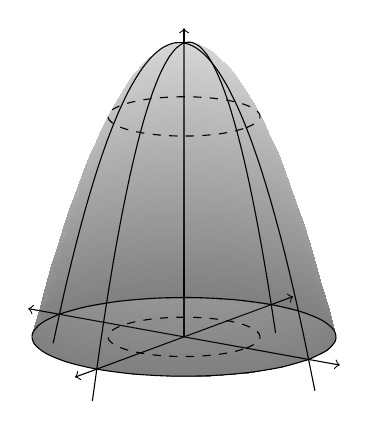
\begin{tikzpicture}
  \begin{axis}[
    view={35}{15},
    unit vector ratio=1 1 1,
    ticks = none,
    axis lines=middle,
    ymin=-2.5,
    ymax=2.5,
    xmax=2.5,
    xmin=-2.5,
    zmin=0,
    zmax=4.2,
    x axis line style=<->,
    y axis line style=<->,
    z axis line style=->,
    clip=false
  ]
    \addplot3[surf,shader=interp,domain=0:360,y domain=0:2, opacity=0.5,
    colormap={blackwhite}{color=(black) color=(black!30)}] ({y*cos(x)},
    {y*sin(x)},{4-y^2});
    \addplot3[samples y=0,domain=0:360,smooth]({2*cos(x)},  {2*sin(x)},0);
    \addplot3[samples y=0,domain=0:360,smooth,dashed]({cos(x)},  {sin(x)},0);
    \addplot3[samples y=0,domain=0:360,smooth,dashed]({cos(x)},  {sin(x)},3);
    \addplot3[samples y=0,domain=-2.1:2.1,smooth](0,  {x},{4 - x^2});
    \addplot3[samples y=0,domain=-2.1:2.1,smooth]({x},0, {4 - x^2});
  \end{axis}
\end{tikzpicture}

We can use polar coordinates to simplify the double integral. In polar 
coordinates, $x = r\cos(\theta)$ and $y = r\sin(\theta)$, so $x^2 + y^2 = r^2$.
The volume under the surface and above the $xy$-plane is given by

\begin{equation}
V = \int \int (4 - r^2) r \, dr \, d\theta,
\end{equation}

where $r$ ranges from 0 to 2 (since $4 - r^2 \geq 0$ if $0 \leq r \leq 2$) and 
$\theta$ ranges from 0 to $2\pi$.

Hence,

\begin{align*}
V & = \int_{0}^{2\pi} \int_{0}^{2} (4r - r^3) \, dr \, d\theta \\
& = \int_{0}^{2\pi} \left[ 2r^2 - \frac{1}{4}r^4 \right]_{0}^{2} \, d\theta \\
& = \int_{0}^{2\pi} (8 - 4) \, d\theta \\
& = \int_{0}^{2\pi} 4 \, d\theta \\
& = \left[ 4\theta \right]_{0}^{2\pi} \\
& = 8\pi.
\end{align*}

So, the volume of the solid is $8\pi$ cubic units.

\end{Answer}

\begin{Exercise}[title = {The volume of a pool}, label = polarmulti2]
A circular swimming pool has a 40-ft diameter. The depth of the pool is 
constant along the north-south axis and increases from 3 feet at the west end 
to 10 feet at the east end. What is the total volume of water in the pool? 
\vspace{50mm}
\end{Exercise}

\begin{Answer}[ref = polarmulti2]
Let us describe the footprint of the pool as a 20-foot radius circle centered 
at the origin (that is, a region $\textit{D} = \{(r, \theta)\text{ }|\text{ }0 
\leq r \leq 20,\text{ }0 \leq \theta \leq 2\pi\}$). Further, let us take 
north-south as parallel to the y-axis and east-west as parallel to the x-axis. 
So, the depth of water is then given by $z = f(x, y) = \frac{7}{40}x + \frac{
13}{2}$ over the footprint of the pool. The total volume of water is given 
by:
$$\int_0^{2\pi} \int_0^{20} r \left( \frac{7}{40}r\cos{\theta} + \frac{13}{2} 
\right)\,dr\,d\theta$$
$$= \int_0^{2\pi} \int_0^{20} \left[ \frac{7}{40}r^2\cos{\theta} + \frac{13}{2}
r \right] \,dr\,d\theta$$
$$= \int_0^{2\pi} \left[ \frac{7\cos{\theta}}{40}\int_0^{20} r^2\,dr + \frac{13
}{2} \int_0^{20} r\,dr \right]\,d\theta$$
$$= \int_0^{2\pi} \left[ \frac{7\cos{\theta}}{40} \left( \frac{1}{3}r^3 \right)
_{r = 0}^{r = 20} + \frac{13}{2} \left( \frac{1}{2}r^2 \right)_{r = 0}^{r = 20}
\right]\,d\theta$$
$$= \int_0^{2\pi} \left[ \frac{1400}{3}\cos{\theta} + 1300 \right]\,d\theta = 
\left[ \frac{1400}{3}\sin{\theta} + 1300\theta \right]_{\theta = 0}^{\theta = 
2\pi}$$
$$= 2600\pi \text{ cubic feet}$$    
\end{Answer}
